\chapter{Data Analysis}

The data analysis focuses, in the first section \ref{cap:Preliminary}, on the preliminary study conducted to understand the feasibility to estimate respiratory rate from a pressure sensor mattress. The data involved in the first part belong to the Sensomative mattress (Chapter \ref{cap:SensomativePar}), collected by a supervisor of this thesis, Manuel Fujis \cite{ManuelZurich}, who kindly make them available.
During the second section \ref{cap:pipeline} is presented the pipeline to analyse the data extracted with the data collection. This pipeline aims to find the best channels, that represent a respiratory pattern, in the mattress and from them estimate the respiratory rate per minute.




%%%%% PRELIMINARY STUDY %%%%%
\section{Preliminary Study on Sensomative Mattress} \label{cap:Preliminary}

A preliminary study on the feasibility of estimating breathing rate from a mattress is conducted on a subsect of the available data belonging to Sensomative mattress (Chapter \ref{cap:SensomativePar}).

From the comparison of raw mattress data and nasal pressure (PSG), as shown in Figure \ref{fig:breathPresent}, is possible to retrieve a respiratory pattern. This is the starting point of the preliminary study.\\


\begin{figure}[H]
    \centering   
    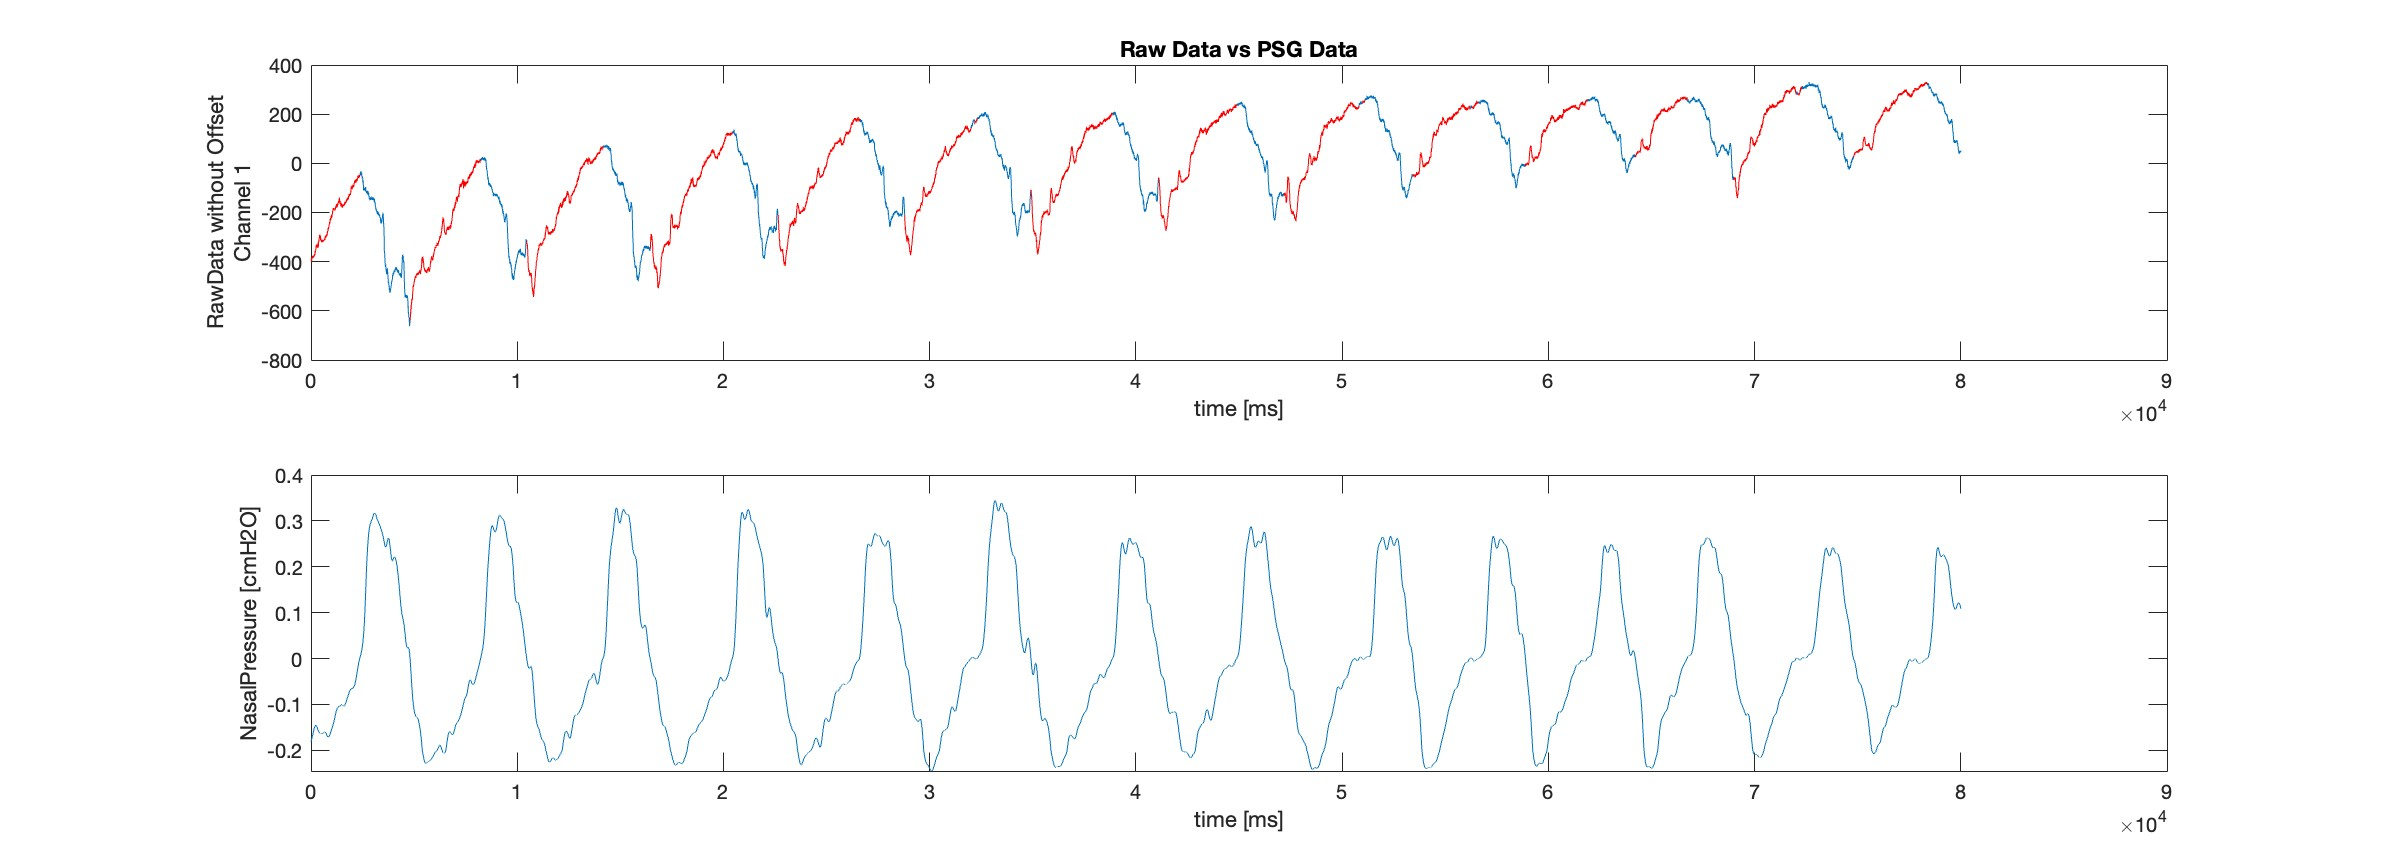
\includegraphics[width=\textwidth]{img/breath_presentation.jpg}
    \caption{Breath pattern}
    \label{fig:breathPresent}
\end{figure}

\vspace*{0.5cm}

The moment between inhaling and exhaling, visible as a peak in the raw data and the PSG data, is counted as a breath. The raw data are too noisy to be given as input to a peak finder, for this reason, is applied a multiresolution overlap discrete wavelet transform, explained later in Chapter \ref{Wavelet}.

\vspace*{0.5cm}

\begin{figure}[H]
    \centering    
    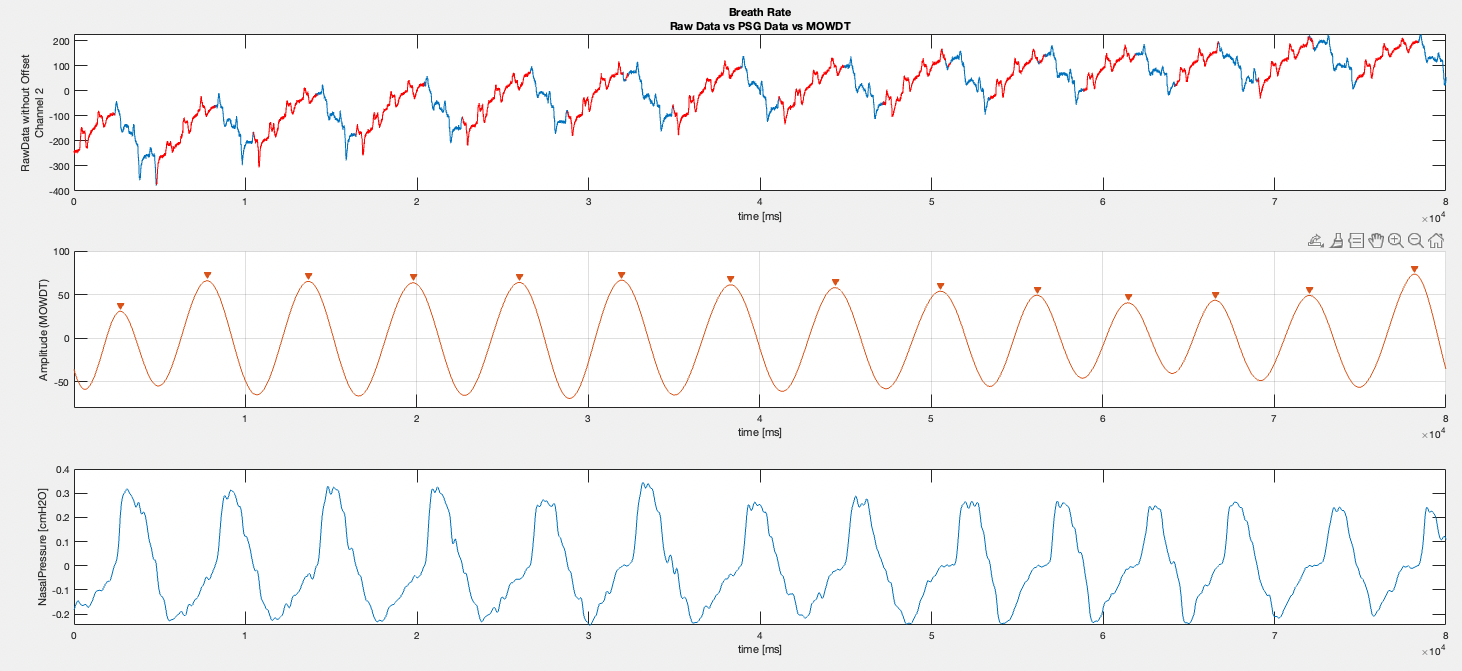
\includegraphics[width=\textwidth]{img/sensomative_manu.png}
    \caption{MODWTMRA reconstruction}
    \label{fig:seonsmativeDataManu}
 
\end{figure}

The so reconstruct signal is given as input to a peak finder that allows counting them and obtaining the respiration rate per minute (rpm).

%%%%% PIPELINE %%%%%
\section{Pipeline}\label{cap:pipeline}
The designed pipeline aims to replicate a semi-realtime analysis using the data obtained from the SensingTex mattress, during the data collection. \newline

The SensingTex has a total number of sensors of 1056, and consequently, the same number of signals from the mattress; this leads to the necessity of an algorithm to discriminate the ones from whom it is possible to extract valuable information about the respiratory rate of the person on the mattress. A person's body can not cover the entire mattress and activate all sensors (hereafter referred to as “Channels”) simultaneously.
Many of these channels present a signal that is stationary on a value; others present just interference from the mattress. From just a few sensors, it is possible to retrieve a respiratory pattern and extract the respiratory rate per minute (rpm). Therefore becomes necessary to design a metric that underlines these channels. The meaning of this metric must be interpreted as confidence expressed as the goodness of the signal in percentual.

Since the designed pipeline aims to replicate a semi-realtime analysis, it takes in input a sliding window of 60 seconds that is moving, for each position, through the 4-minute recording obtained after the cleaning of the data (Chapter \ref{cap:dataProcessing}). Figure \ref{fig:recordingCut4} shows a 4-minute recording with a highlighted window of 60 seconds, which can be consulted in more detail in figure \ref{fig:recordingCut1}.

\vspace{0.5cm}

\begin{figure}[h]
    \centering    
    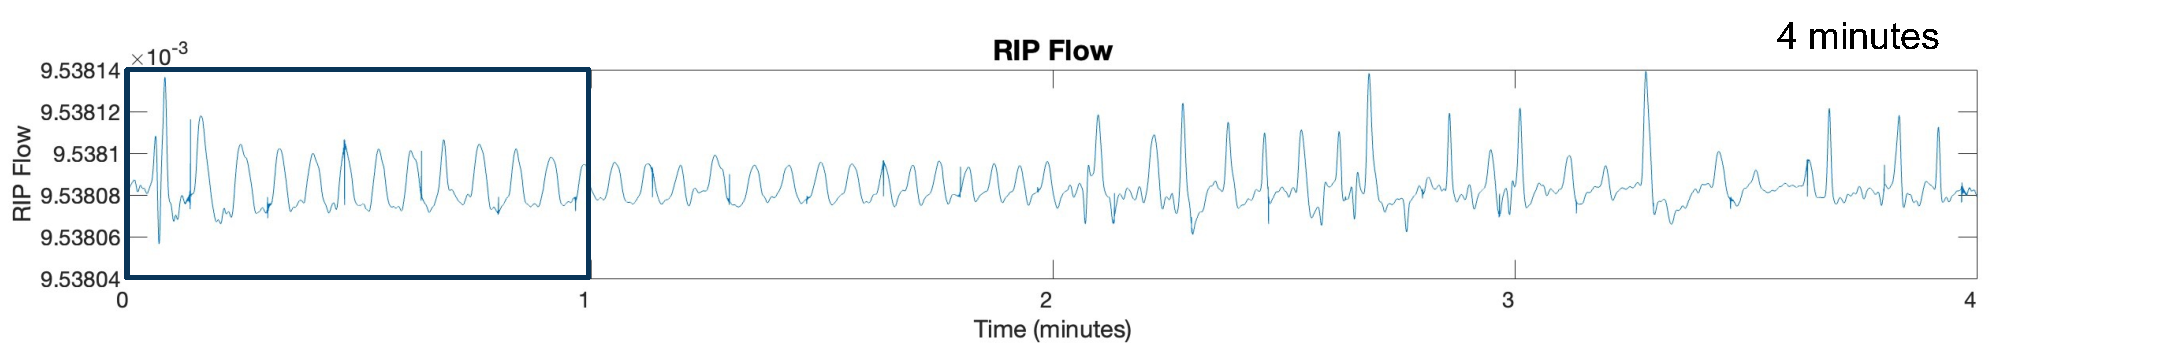
\includegraphics[width=\textwidth]{img/4minute.pdf}
    \caption{4 minute}
    \label{fig:recordingCut4}
\end{figure}
\vspace{0.7cm}
\begin{figure}[h]
    \centering
    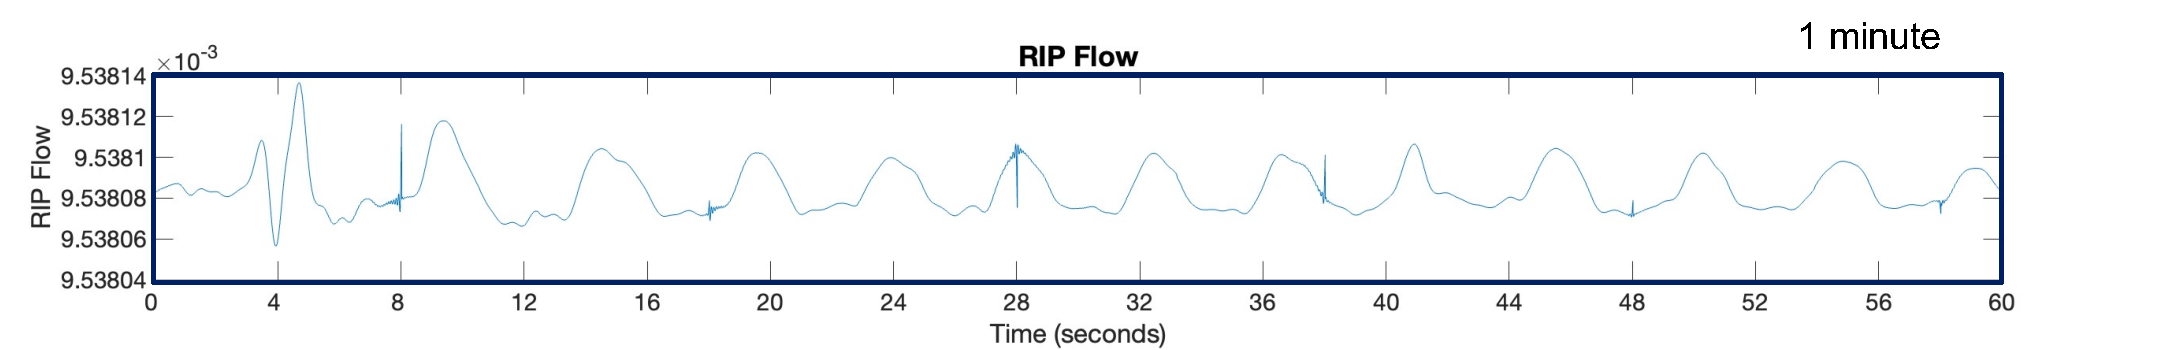
\includegraphics[width=\textwidth]{img/1minute.pdf}
    \caption{1 minute}
    \label{fig:recordingCut1}
\end{figure}

In Figure \ref{fig:pipeline} it is possible to visualize a scheme of the entire pipeline.

\begin{figure}[p]
    \centering
    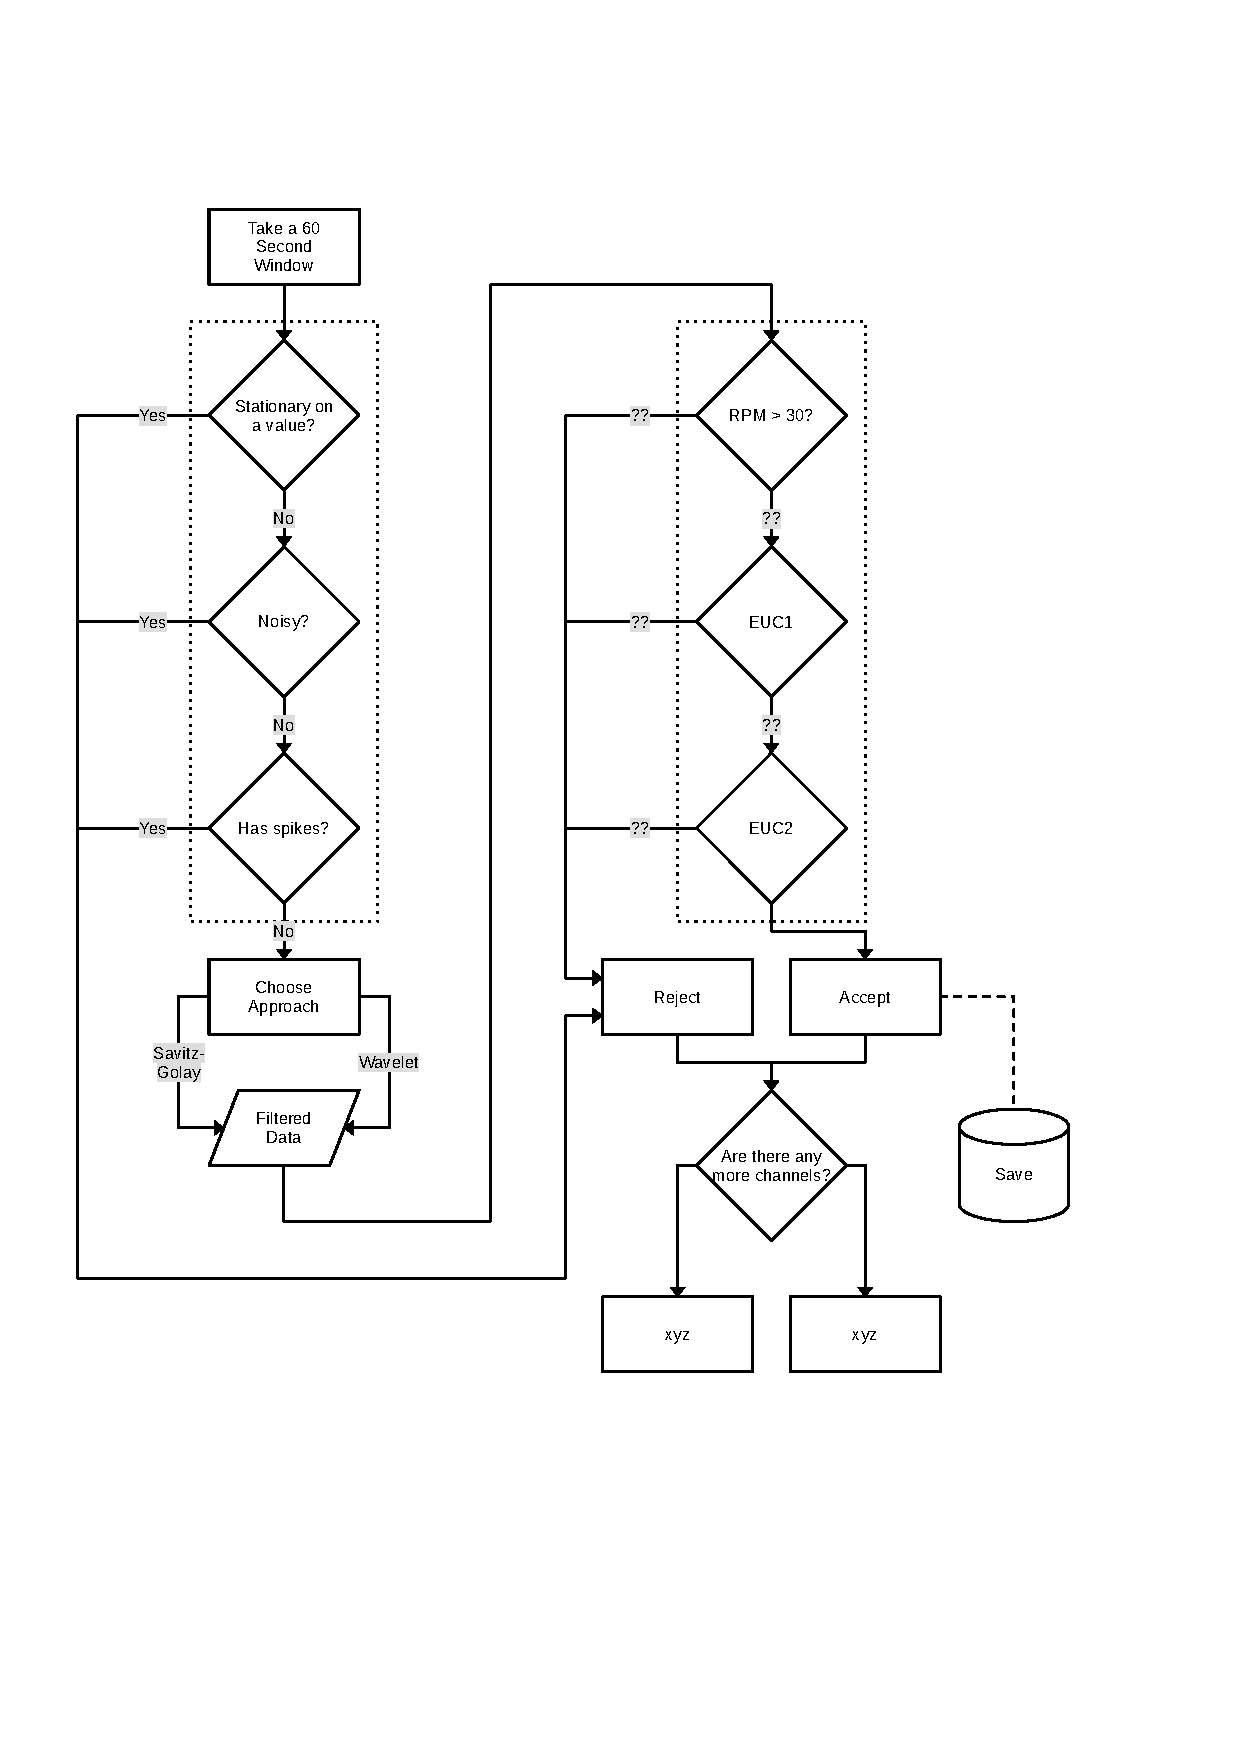
\includegraphics[width=0.9\textwidth]{img/pipeline.pdf}
    \caption{Pipeline}
    \label{fig:pipeline}
\end{figure}

\subsection{Weighted and binary method}
The metric has been designed as a confidence expressed as the goodness of the signal in percentual. To create this percentual has been decided to use create a series of criteria that each signal has to follow. 

Some of these criteria, such as in Chapter \ref{cap:excCrit}, are excluding criteria, that are referred to particular phenomena that if present for the entire length lead to having an unusable signal.
If one of these criteria is not passed the signal is not further analysed, but if they present the phenomena but not for the entire length, it has been decided to keep them and understand if in another part they could be meaningful. So they can express the percentage of the signal that follow those criteria or just that they present a possible meaningful part. 

For this reason, it has been implemented a version of the pipeline where the criteria are binary, they can be passed or not (1 passed, 0 not passed), and a version where some criteria give as an answer the percentage of the channel that could contain valuable information (hereafter also referred to as "weighted method"). For each criterion, the following section will explain the different outputs of the metrics, in the case of binary or weighted approach.
In both cases, the final confidence is the mean of percentages of each criterion.


\subsection{Excluding criteria}\label{cap:excCrit}
The first step of this pipeline excludes those signals for the entire window length that is stationary on value, with small amplitude, or present only interference from the mattress. So channels do not have meaningful information, in case this behaviour is present in a part of the signal the output for the metric is different based on the binary or weighted approach. Artefacts are the only excluding criteria.

\subsubsection*{Stationary signals on a value}\label{cap:stationary}
A stationary signal on a value is defined as a signal that remains on the same value for the entire length of the window.

An example of the stationary signal on a value is shown in Figure\ref{fig:stationaryTotal}, in this case, the channel, for this window, is excluded and not further analysed.
However, since it is used as a moving window it will take again into account in the next window and, if it presents a different behaviour, it maybe is considered. 
Nevertheless, If the channel presents only a part of the signal stationary on a value as in Figure\ref{fig:spikePartial}, the channel is given as a percentage of confidence, the percentage of the non-stationary on a value signal for weighted approach or 1 for binary if the non-stationary value is more than 20\%.
\vspace*{0.5cm}
\begin{figure}[H]
    \centering
    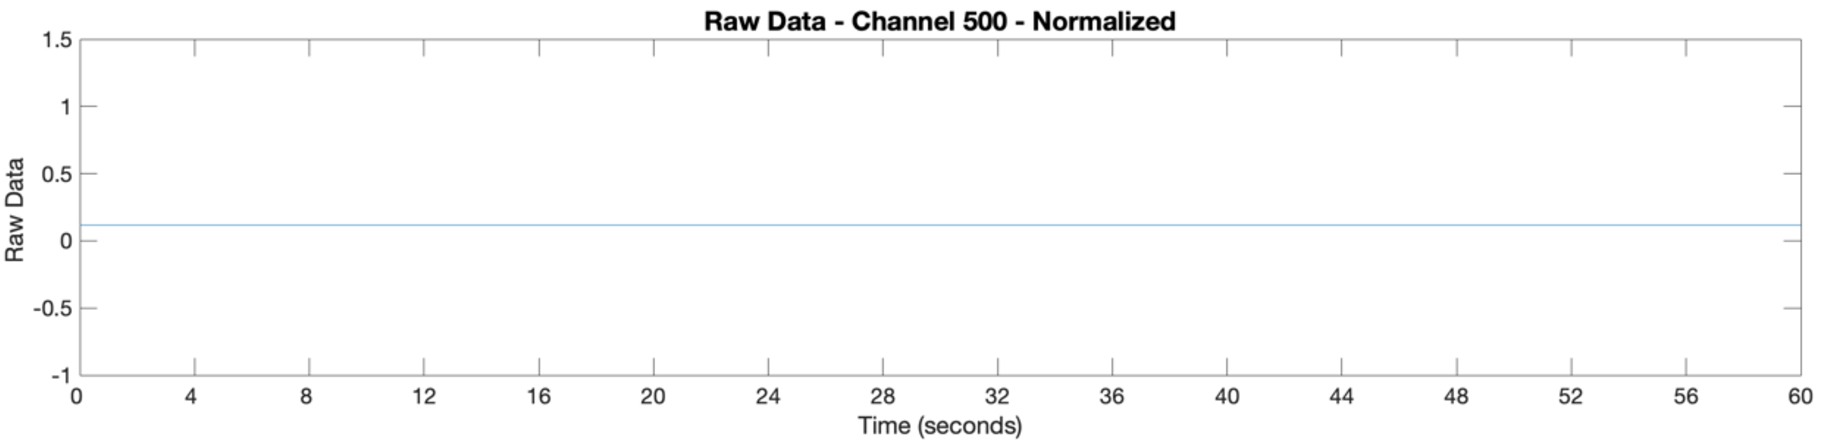
\includegraphics[width=\textwidth]{img/stationary.pdf}
    \caption{Raw Data - Channel 500 -  Stationary on a Value}
    \label{fig:stationaryTotal}
\end{figure}
\vspace*{0.5cm}
\begin{figure}[H]
    \centering
    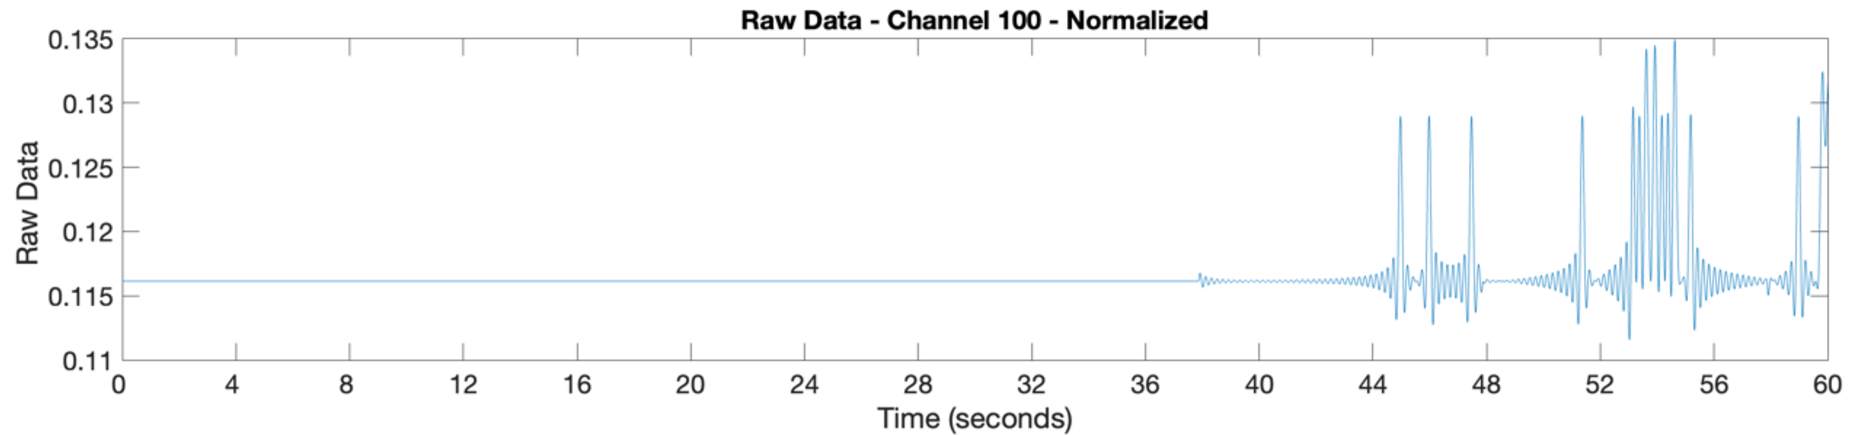
\includegraphics[width=\textwidth]{img/spakePartial.pdf}
    \caption{Raw Data - Channel 100 - Partial Stationary Signal}
    \label{fig:spikePartial}
\end{figure}

\subsubsection*{Signal with small amplitude}\label{cap:noisy}

Several channels present a signal with a small amplitude, between [intervall], an example is visible in Figure \ref{fig:noisy}, so after verifying if they are not stationary on a value case (Chapter \ref{cap:stationary}), if the signal presents a small amplitude for the entire length of the window that could not represent a respiratory pattern is excluded. 
Otherwise, if part of the signal does not have a small amplitude: for the weighted approach, the percentage of confidence in output is equal to the percentage of a signal without a small amplitude.; for the binary approach, the criteria is passed if the small amplitude is present in less than 20\% of the signal.
As in the previous case, due to the moving window nature of the pipeline after the shift of 10 seconds, the channel could have a different behaviour and be further analysed.\\


%\vspace*{1.0cm}
\begin{figure}[H]
    \centering
    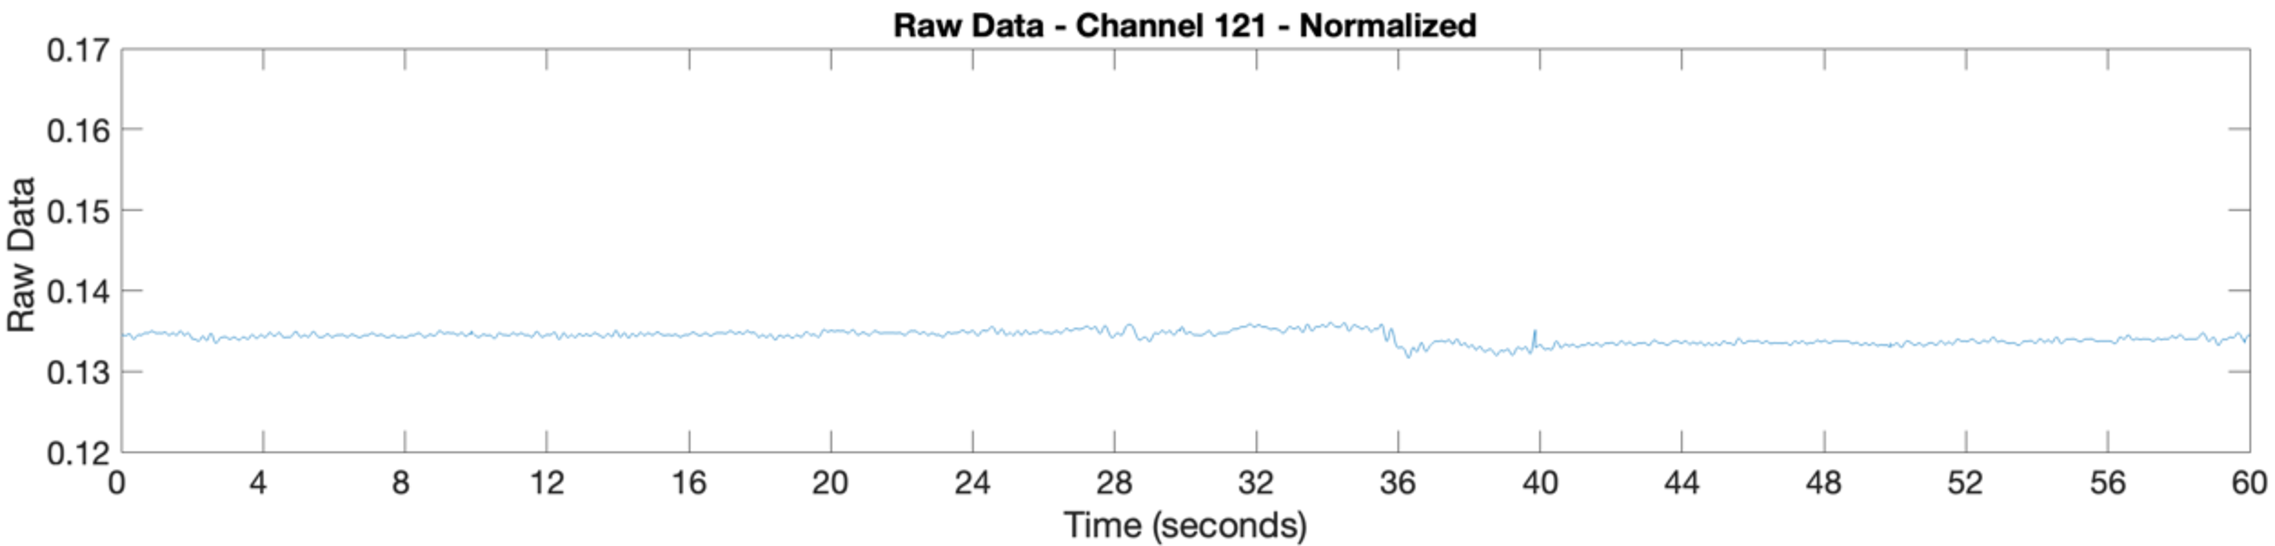
\includegraphics[width=\textwidth]{img/noisy.pdf}
    \caption{Raw Data - Channel 121 - Small amplitude}
    \label{fig:noisy}
\end{figure}


\subsubsection{Spikes Signals} \label{spikes}
The mattress can produce artefacts, that are visible in the channels as spikes as in Figure \ref{fig:spikeTotal}. 
Since these artefacts are visible also in channels that present a good respiratory pattern (Figure \ref{fig:goodSignal}), after evaluating different thresholds it has been decided to accept the channel that has a percentage of spikes under 30\%. In this case, both methods (binary and weighted), has the same output 100\% or 1 in case of passed criteria, 0 otherwise.\\


\begin{figure}[H]
    \centering
    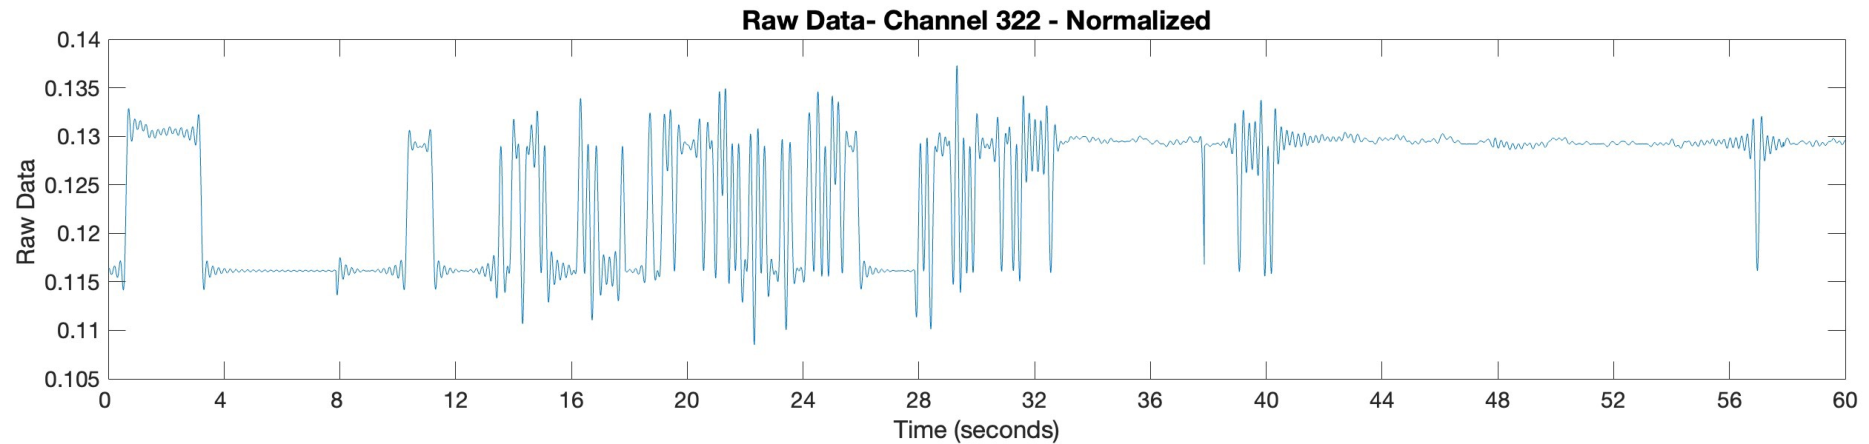
\includegraphics[width=\textwidth]{img/spike_total.pdf}
    \caption{Raw Data - Channel 322 - Massive presence of Spike}
    \label{fig:spikeTotal}
\end{figure}

\begin{figure}[H]
    \centering
    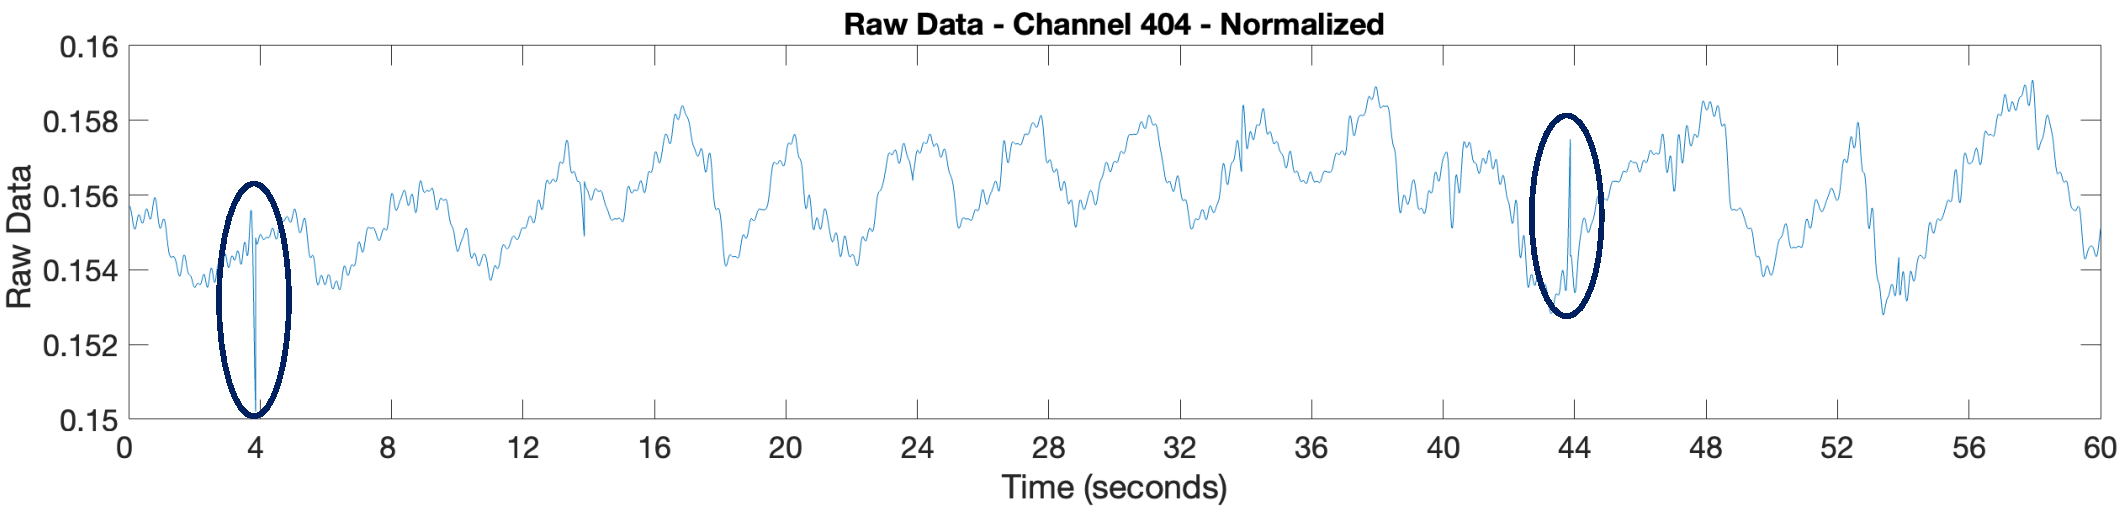
\includegraphics[width=\textwidth]{img/goodSpikes.pdf}
    \caption{Raw Data - Channel 404 - Small presence of spikes}
    \label{fig:goodSignal}
\end{figure}

\subsection{Denoised Signals}
After these preliminary analyses, the number of signals decreases drastically; as a result, has been obtained signals that could contain valuable information and the relative percentage of confidence.
To be able to estimate the number of breaths it has been assumed to count as one breath the moment between inhale and exhale, which can also be considered a peak in the signal.
At this point, most of the signals are still noisy. To be better analysed has been decided to filter them. In general, filtering consists of replacing each point of a signal with some combination of the signal values contained in a moving window centred at the point, on the assumption that nearby points measure nearly the same underlying value.

In this pipeline two different kinds of approaches are involved: Multiresolution analysis of the maximal overlap discrete wavelet transform (Chapter \ref{Wavelet}), and Savitz-Golay filter (Chapter \ref{sg}).
It is possible to choose which approach to use in the context of the data, in this project are both used rather than compare them.


%%%%%%%% WAVELET %%%%%%%%
\subsection{Multiresolution Overlap Discrete Wavelet Transform} \label{Wavelet}

The Multiresolution Overlap Discrete Wavelet Transform (hereafter also referred to as "MODWTMRA") is based on wavelet analysis (MOWDT) that transforms the original signal into a time-frequency domain to be analysed and processed, the multiresolution analysis (MRA), which cuts the signal into components, can produce the original signal exactly when added back together.

The input data of MOWDT are samples of a function $f(x)$ evaluated at $N$ time points, this function can be expressed as the linear combination of the scaling function $\phi(x)$ and wavelet $\psi(x)$ at varying scales and translations:

$$f(x)=\sum_{k=0}^{N-1} c_k 2^{-J_0/2} \phi(2^{-J0}x-k) + \sum_{j=1}^{J_0}f_j(x)$$
where 

$$f_j(x)=\sum_{k=0}^{N-1} d_{j,k}2^{-J/2} \phi(2^{-J}x-k)$$

and $J_0$ is the number of levels of wavelet decomposition calculated as $floor(log_2(N))$.

The first sum represents the first approximation of the signal and then the successive scales.
MODWT returns the $N$ coefficients $\{c_k\}$ and the $(J_0 $ X $ N)$ detail coefficients $\{d_{j,k}\}$ of the expansion. 

Since it has been used the MODWTMRA, instead of just MODWT, the returns are the projections of the function $f(x)$ onto the various wavelet subspaces and final scaling space. That is, MODWTMRA returns 
$$\sum_{k=0}^{N-1} c_k 2^{-J_0/2} \phi(2^{-J0}x-k)$$\newline
and the $J_0$-many $\{f_j(x)\}$ evalutaed at $N$ time points.
It is then obtained a projection of $f(x)$ onto a different subspace, the original signal can be recovered by adding all the projections. 

For our approach, we choose the Daubechies wavelet with two vanishing moments (Figure \ref{fig:Daubechies}) that better represent the breath signal present in our data.

\begin{figure}[h]
    \centering
    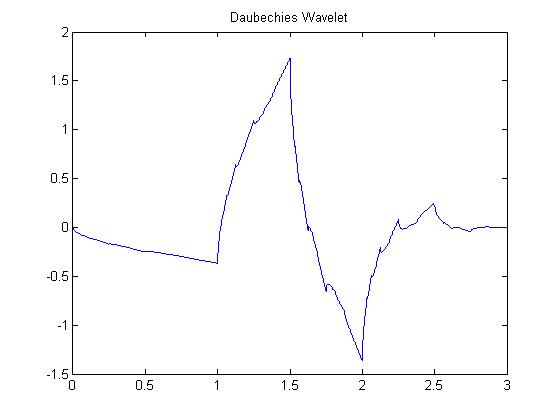
\includegraphics[width=0.6\textwidth]{img/gooddb.jpeg}
    \caption{Daubechies wavelet with two vanishing moments}
    \label{fig:Daubechies}
\end{figure}


The decomposition of the signal of channel 404 (Figure \ref{fig:404}), is shown in Figure \ref{fig:level1}. The raw data has been decomposed into 13 levels to obtain our denoised signal, it has been decided to sum only a subset of this scale, which allowed us to reconstruct a clear signal where the peaks could be underlined and counted. 

\begin{figure}[p]
    \centering
    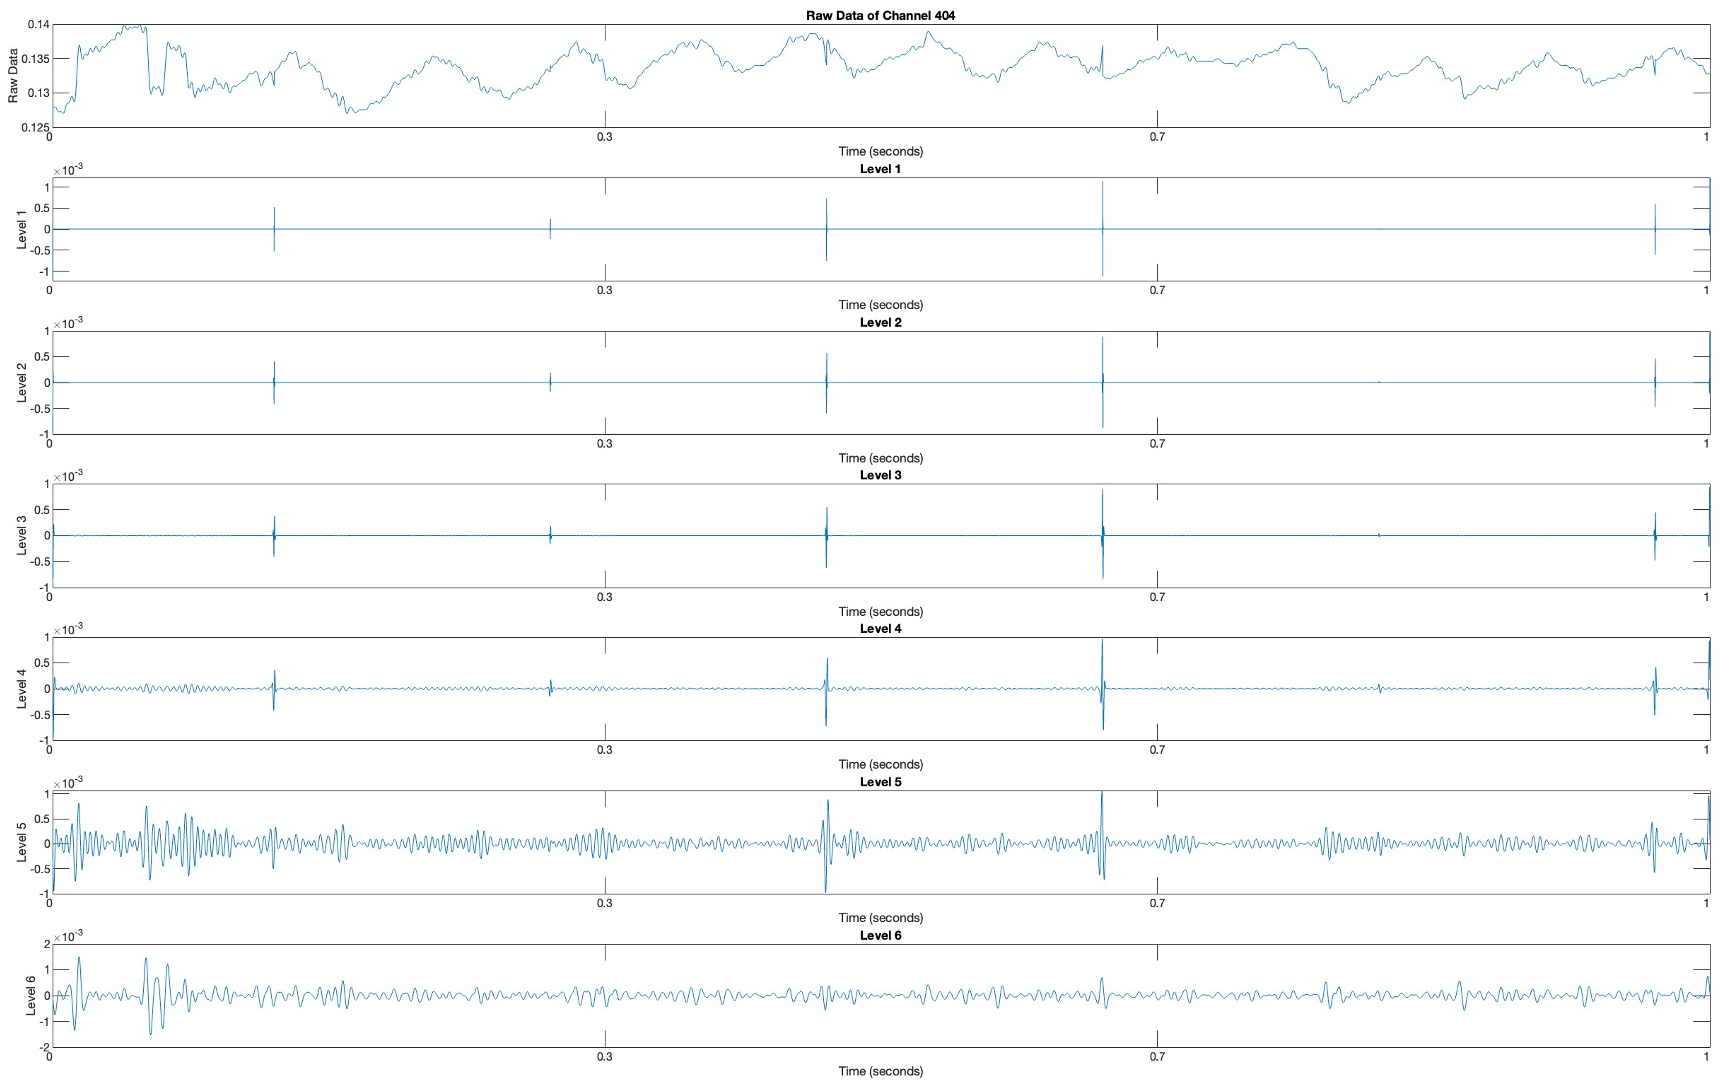
\includegraphics[width=\textwidth]{img/lev1.png}
    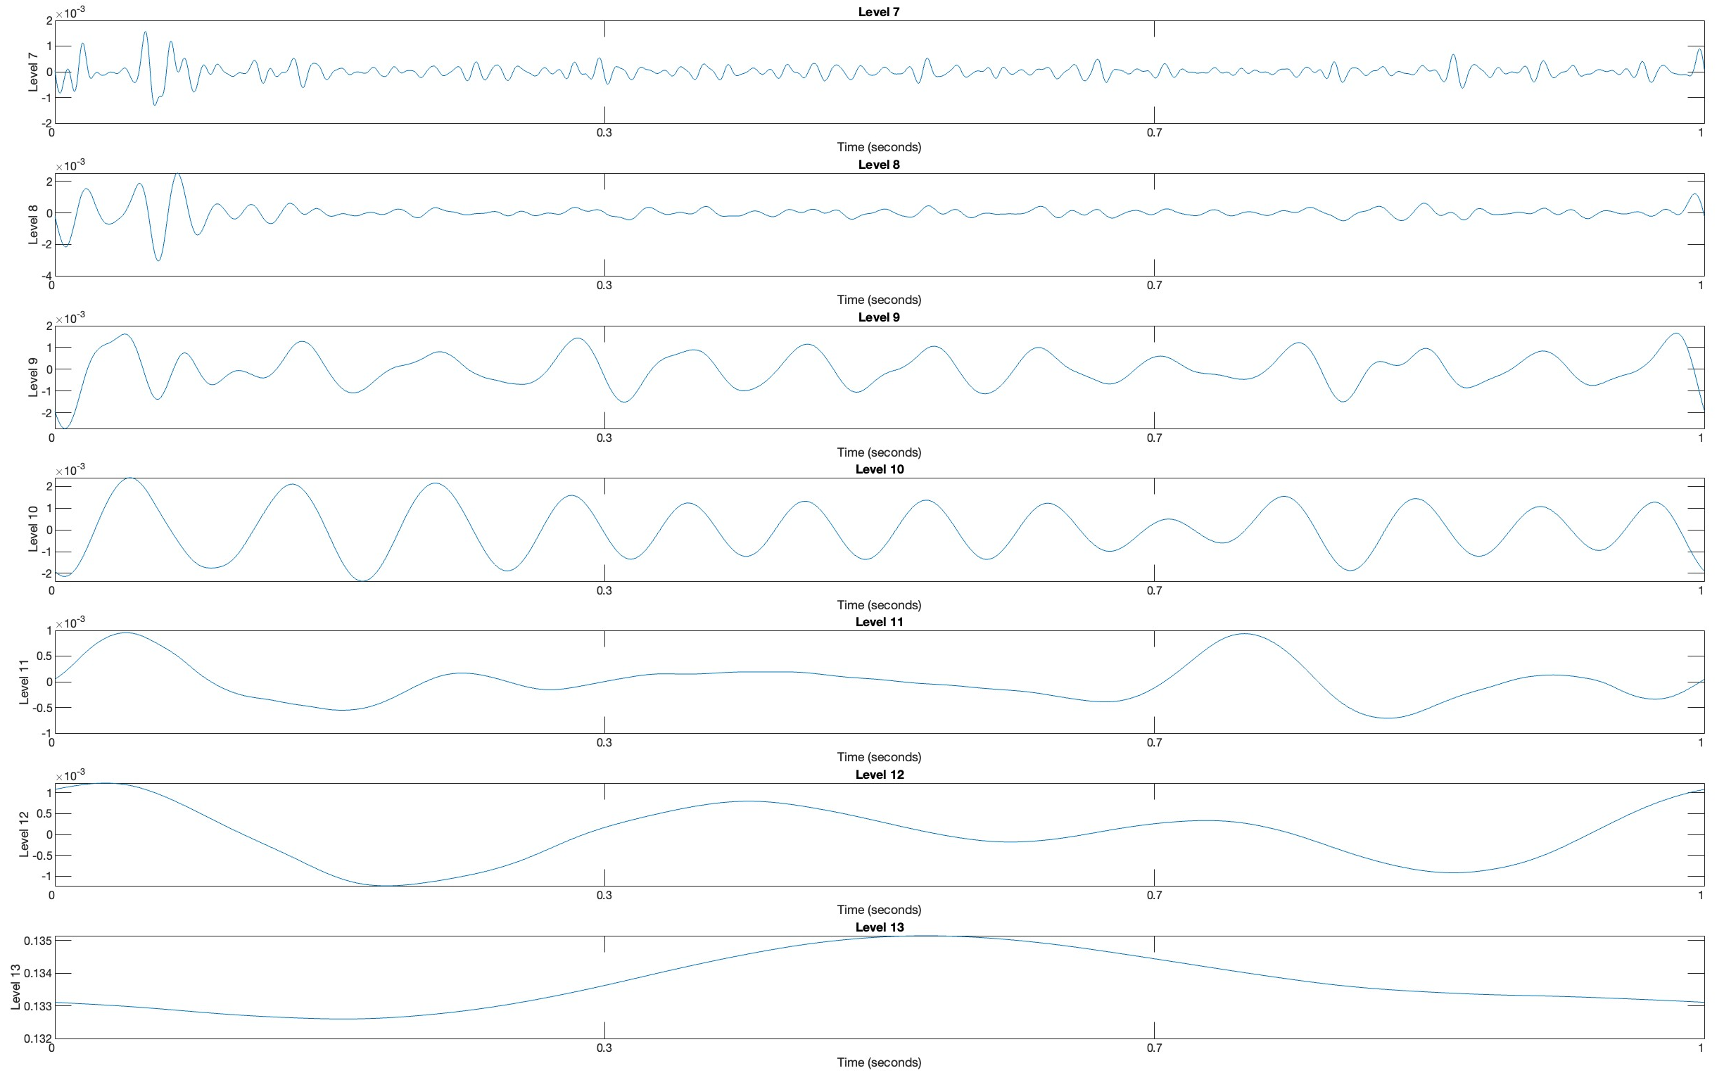
\includegraphics[width=\textwidth]{img/lev2.png}
    \caption{Stationary Signal}
    \label{fig:level1}
\end{figure}

%%%%%  APPLICAZIONE WAVELET %%%%%
\subsubsection{Application in the Pipeline}
To show the application of the MOWDTMRA in the pipeline, the signal in Figure \ref{fig:404}, which has not been excluded by the criteria explained in Chapter \ref{cap:excCrit} is taken as an example.

The signal is decomposed in 13 levels, as shown in Figure \ref{fig:level1}, and choose the levels that are added together to reconstruct the signal of breath rate, in the context of this project the $9^{th}$ and $10^{th}$ level. The levels are chosen to recreate a wave that best fits the original wave of the signal but excludes the noise.
The resulting wave is given as input to a peak finder to point out the moment between inhaling and exhaling, visible as a peak in the wave and counted as a breath. Since the window is 60 seconds long, these peaks are interpreted as rpm. The resulting plot is shown in Figure \ref{fig:404Filt}.
\begin{figure}[H]
    \centering
    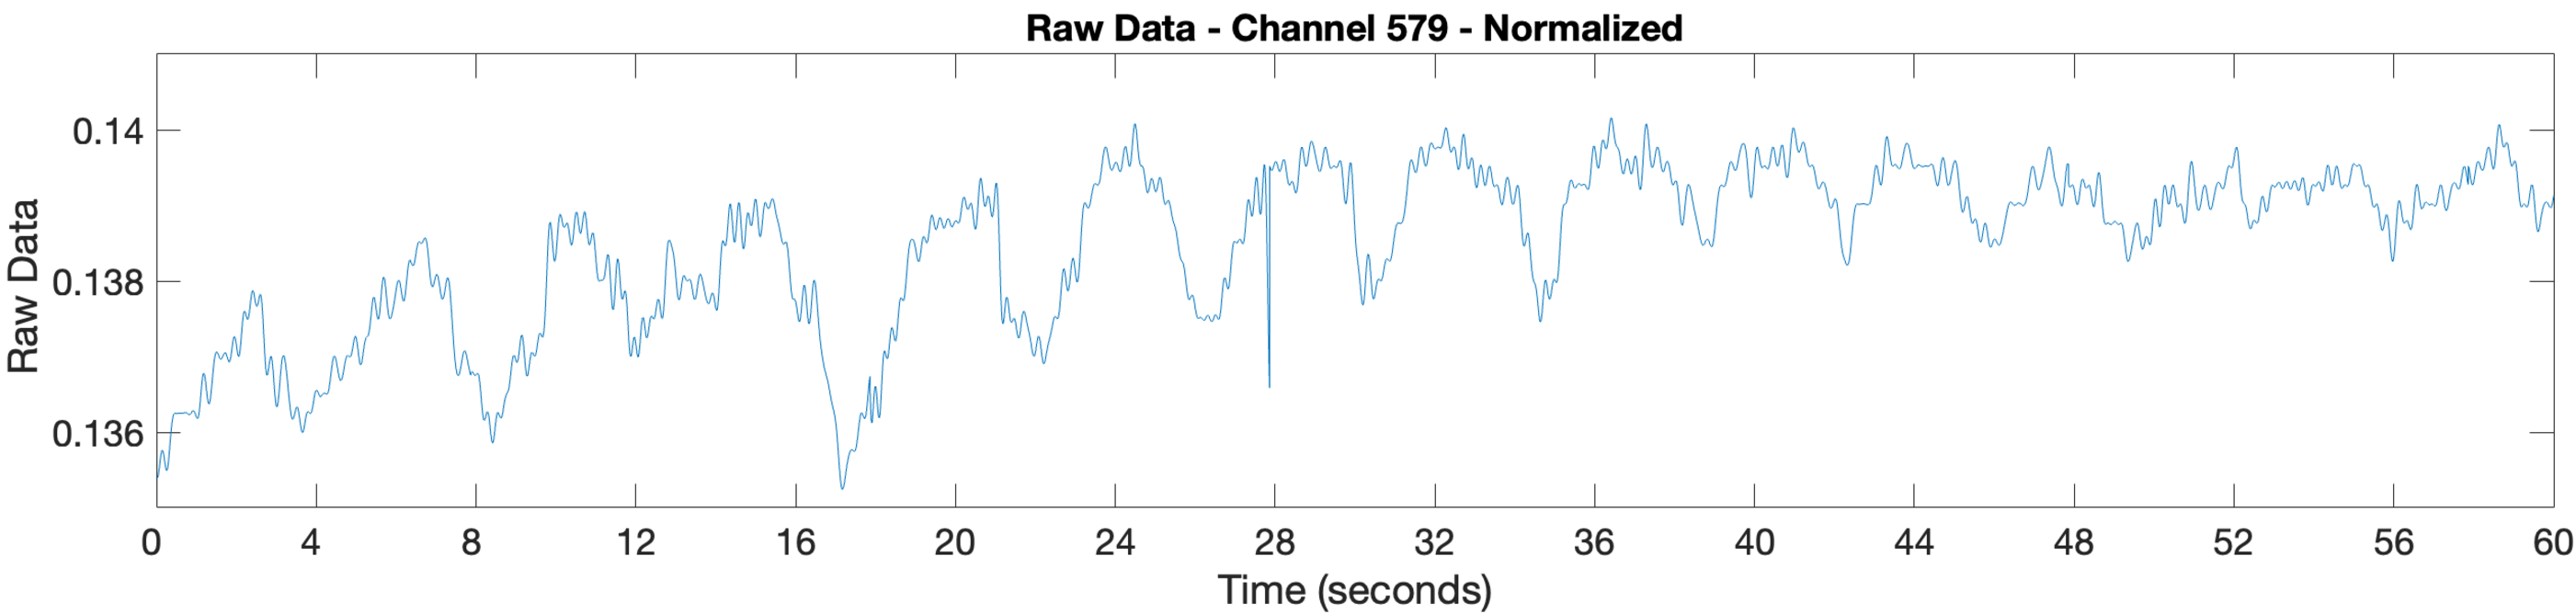
\includegraphics[width=\textwidth]{img/579.pdf}
    \caption{Raw Data - Channel 579 - Massive presence of Spike}
    \label{fig:404}
\end{figure}

\begin{figure}[H]
    \centering
    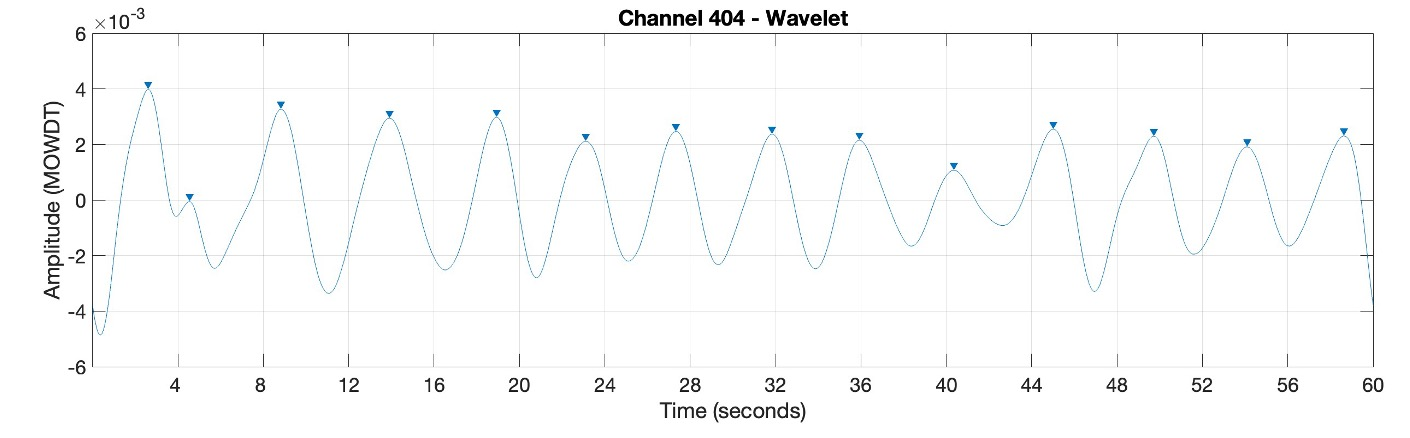
\includegraphics[width=\textwidth]{img/404_wave.jpg}
    \caption{Channel 404 Filtered - with Wavelet}
    \label{fig:404Filt}
\end{figure}


%%%%%  Savitz-Golay  %%%%%
\subsection{Savitz-Golay filter} \label{sg}


The Savitz-Golay filter is a filter used to "smooth out" a noisy signal whose frequency span (without noise) is significant. 
They are also called digital smoothing polynomial filters or least-squares smoothing filters. 
Savitzky-Golay filters generalize the idea of filtering of replacing each point of a signal with a combination of the signal values contained in a moving window centred at the point, on the assumption that nearby points measure nearly the same underlying value, by least-squares fitting an $n$th-order polynomial through the signal values in the window and taking the calculated central point of the fitted polynomial curve as the new smoothed data point.

For a given point $\textbf{x}$ that has $k$ points to the left and $k$ points to the right, for a total window length of $L = 2k + 1$:
\vspace*{0.5cm}

$$\textbf{x}= 
\begin{bmatrix}
    1 & -k & (-k)^2 & \cdots & (-k)^n\\ 
    1 & \vdots &\vdots & \ddots & \vdots\\  
    1 & -2 & (-2)^2 & \cdots & (-2)^n\\  
    1 & -2 & (-1)^2 & \cdots & (-1)^n\\  
    1 & 0 & 0 & \cdots & 0\\   
    1 & 1 & 1^2 & \cdots & 1^n\\   
    1 & 2 & 2^2 & \cdots & 2^n\\    
    1 & \vdots &\vdots & \udots & \vdots\\   
    1 & k & k^2 & \cdots & k^n\\   
  \end{bmatrix}
  \begin{bmatrix}
    a_0\\ 
    \vdots \\  
    a_n 
  \end{bmatrix}
\equiv
  \textbf{Ha}
  $$
  \vspace*{0.5cm}


  To find the Savitzky-Golay estimates, use the pseudoinverse of $\textbf{H}$ to compute a and then premultiply by $\textbf{H}$
  \vspace*{0.5cm}

$$
\hat{\textbf{x}} = \textbf{H}(\textbf{H}^\textit{T}\textbf{H})^{-1}\textbf{H}^\textit{T}\textbf{x} = \textbf{Bx} 
$$ 

\vspace*{0.5cm}

An example of how the Savitzky–Golay filter works is shown in Figure \ref{fig:4sg explain}.

\begin{figure}[p]
    \centering
    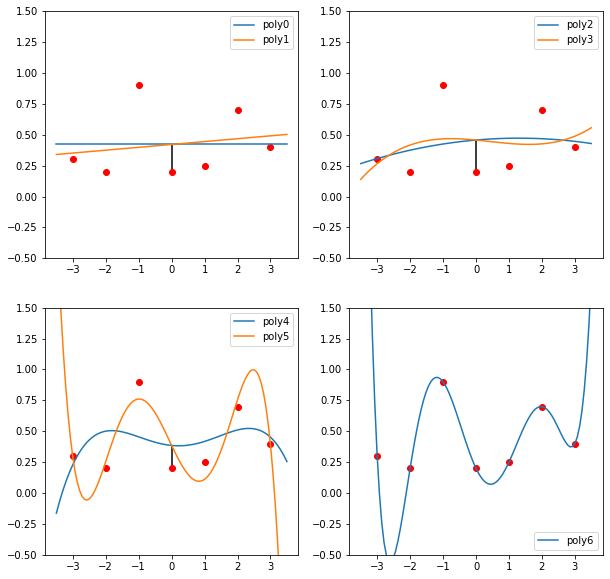
\includegraphics[width=\textwidth]{img/sg_expl.png}
    \caption{Savitzky-Golay filter}
    \label{fig:4sg explain}
\end{figure}
\clearpage



\subsubsection{Application in the Pipeline}

To show the application of the Savitz-Golay filter in the pipeline, the signal in Figure \ref{fig:404}, which has not been excluded by the criteria explained in Chapter \ref{cap:excCrit} is taken as an example.

For the filter is chosen a $9th$ order polynomial, that allows for obtaining a wave similar to the one in MODWTMRA form.
The resulting wave is given as input to a peak finder to point out the moment between inhaling and exhaling, visible as a peak in the wave and counted as a breath and since the window is 60 seconds long, these peaks are interpreted as rpm. The resulting plot is shown in Figure \ref{fig:404sg}.

\vspace*{0.5cm}

\begin{figure}[H]
    \centering
    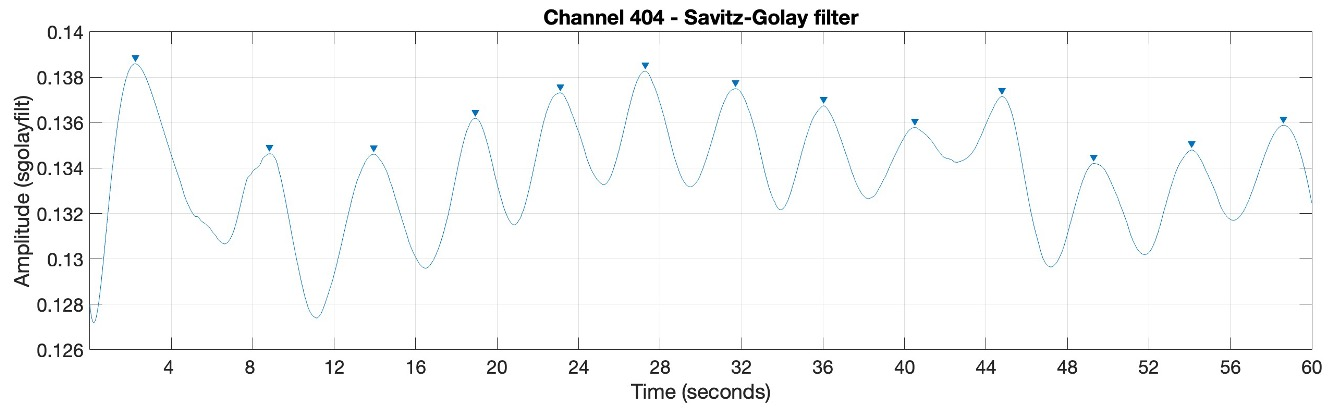
\includegraphics[width=\textwidth]{img/404sg.jpg}
    \caption{Channel 404 Filtered - with Savitz-Golay filter}
    \label{fig:404sg}
\end{figure}

\vspace*{0.3cm}


%\subsection{SNR ratio}

\subsection{Subsequent analyses of the filtered signal}
The reconstructed signal with MODWTMRA or Savitzky–Golay filter is then further analysed, based on physiological information. This criterion is considered binary, so the weighted approach follows the scheme 1000\% in case of passed and 0\% otherwise.

\subsubsection{Respiratory Rate over a Threshold}\label{threshold}
Since this project is a preliminary analysis of the feasibility to use pressure sensor mattresses to estimate a respiratory rate per minute (rpm). It has been decided to choose a threshold over which a respiratory rate of a person should not go %and set an alarm if the rpm goes over it. The choosen 
, threshold is 30rpm because as discussed in Chapter \ref{cap:respiratorySystem} an rpm greater than 20 breaths per min was predictive of cardiopulmonary arrest within 72 hours and death within 30 days\cite{Hong2013HowPatients}; greater than 27 breaths per minute were predictive of cardiopulmonary arrest within 72 hours \cite{Fieselmann1993RespiratoryInpatients}.
So %exclude 
the channels with a signal with more than 30 rpm, to admit a part of the error in our reconstruction and arrive at the limit given by literature between healthy and problematic and lead to a 0\% percentage of confidence.

\subsubsection{Distance peaks valley} \label{cap:Euclidian}
The signal is then given as input to an algorithm that points out the valley of the filtered signal and not only the peaks.
The distance between valley and peaks is calculated with Euclidean distance, if the value between the signal's valley and peaks should differ inside the interval of ±20$\%$ from the preceding breath the signal is considered to be meaningful and lead to a 100\% percentage of confidence.
\vspace*{0.5cm}

\begin{figure}[H]
    \centering
    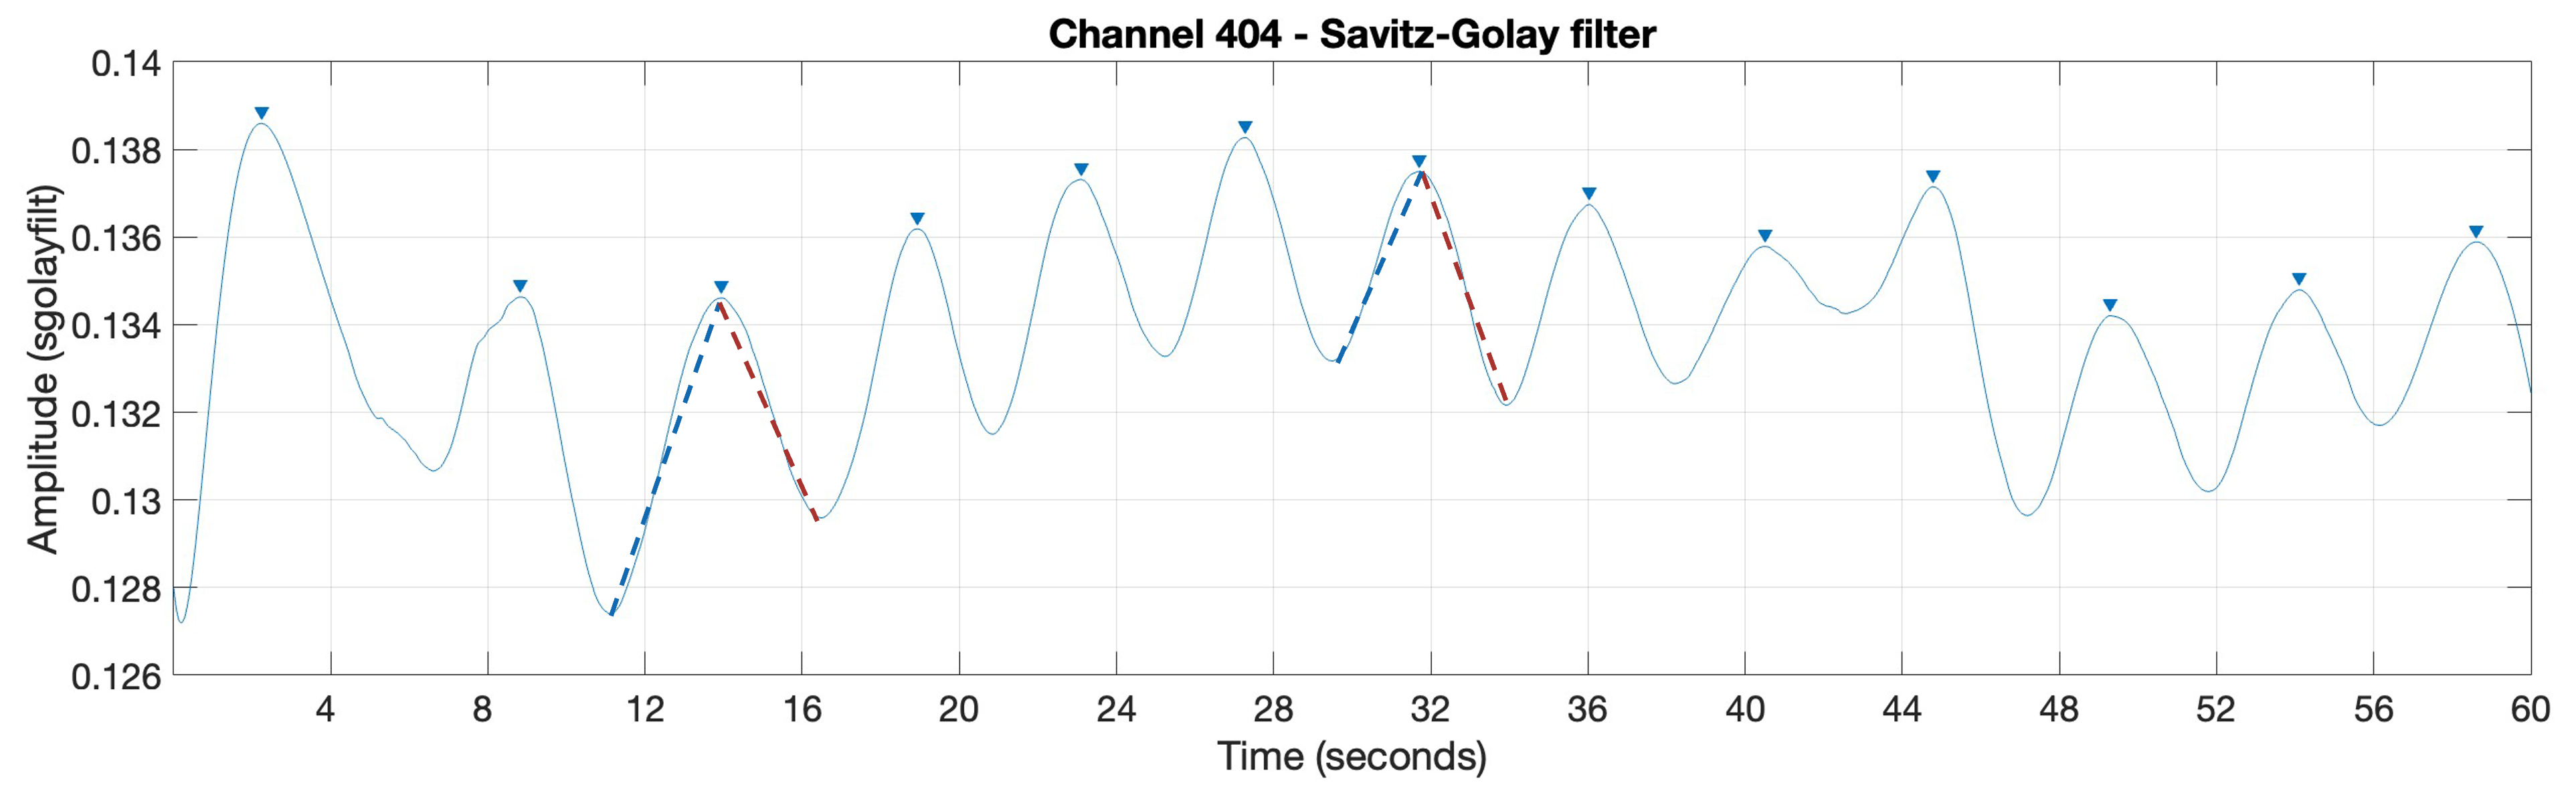
\includegraphics[width=\textwidth]{img/euclidian.png}
    \caption{Euclidean}
    \label{fig:Euclidean}
\end{figure}
\vspace*{0.3cm}

\subsubsection{Lenght of breath} \label{cap:BrethLength}
The valley calculated in Chapter \ref{cap:BrethLength} are taken into account to calculate the distance between peaks and valleys on the time axis, to check the length of inspiration and expiratory phase. The difference should not vary between ±20 \% from the previous breath. If the signal is in this range the channel is considered meaningful and leads to a 100\% percentage of confidence.\\
\vspace*{0.5cm}

\begin{figure}[H]
    \centering
    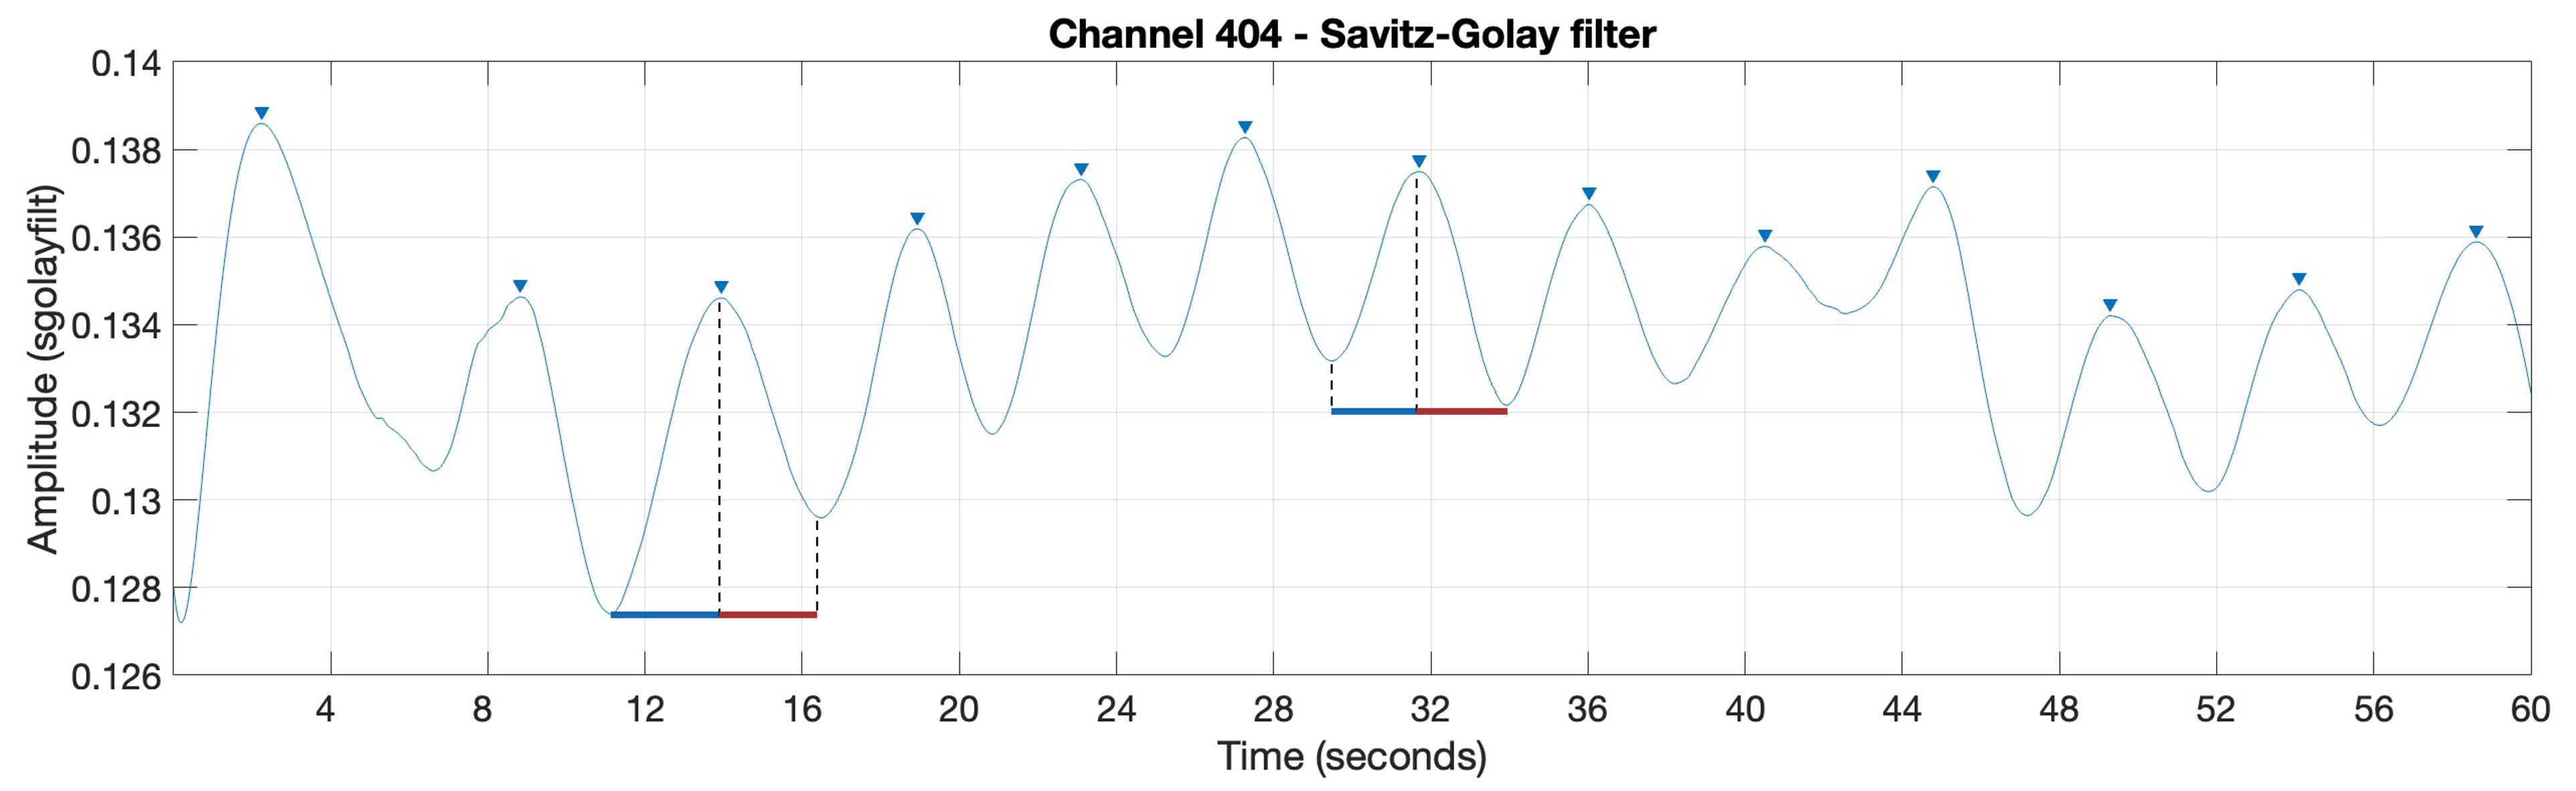
\includegraphics[width=\textwidth]{img/x_axis.png}
    \caption{Length}
    \label{fig:lenght}
\end{figure}
\vspace*{0.3cm}

\subsection{Compute the Respiratory Rate}

At the end of the pipeline, for each method: binary or weighted; for each approach: MODWTMRA and Savitzky–Golay filter, it has been saved the result of each of them. In case it is been decided to perform the approach and methods, there are a total of four combinations:
\begin{itemize}
    \item MODWTMRA filter with a binary approach
    \item MODWTMRA filter with MODWTMRA approach
    \item Savitzky–Golay filter with a binary approach
    \item Savitzky–Golay filter with MODWTMRA approach   
\end{itemize}

In the end, to calculate the rpm, the channels with the highest accuracy, which can be chosened at the beginning of the pipeline, are taken into account, and the rpm is computed as the average of the number of peaks of the signals.

\subsection{Result of the Pipeline (visual)}
As a result, the pipeline is also available a heatmap that allows visualizing where the channels with the highest percentage of confidence, understand where are in respect of the body. Figure \ref{fig:heat}, is an example of the resulting heatmap, where the channels with the highest value are red and with lower are green up to blue when the channels have the 0\% of representing a respiratory pattern.

\begin{figure}[H]
    \centering
    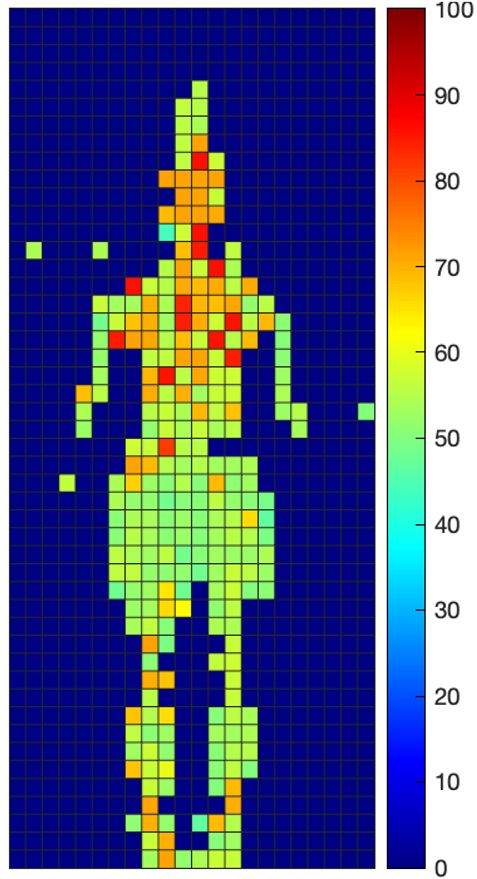
\includegraphics[width=0.65\textwidth]{img/total.png}
    \caption{Heatmap of channels with the highest confidence}
    \label{fig:heat}
\end{figure}
